\documentclass[12p]{article}
\usepackage[utf8]{inputenc}
\usepackage{amssymb}
\usepackage{graphicx}
\usepackage{graphicx}
\usepackage{amsmath}
\usepackage[inkscapeformat=png]{svg}
\usepackage{wasysym}
\graphicspath{ {./images/} }
\usepackage{subcaption}
\usepackage{listings}
\usepackage{csquotes}
\usepackage{wrapfig}
\usepackage[colorlinks, bookmarks=false, linkcolor=black, urlcolor=blue, citecolor=black]{hyperref}
\usepackage{matlab-prettifier}
\usepackage[top=2.5cm, bottom=3 cm, left=3.5cm, right=3.5cm]{geometry}
\usepackage{xcolor}

% \pagecolor{black}
% \color{white}

\newcommand*{\proj}{\text{Proj}}
\newcommand*{\es}{\mathcal{E}}

\title{MATH-329 Nonlinear optimization
Homework 3: Constrained optimization}
\author{Alix Pelletier 346750 \\ Vlad Burca 344876 \\ Ismail Bouhaj 326480}
\date{11/2023}
\begin{document}
\maketitle 
\section*{Part 1 : Projections to cones and stopping criteria in constrained optimization.}
\subsection*{Question 1} \hfil\par
Since \(Q\) is non-empty, Let \(x_0\in Q\). Then by definition of the minimizer, we have:
\[
  \min_{x\in Q} \frac{1}{2}\|x-z\|^2 \leq \frac{1}{2}\|x_0-z\|^2
\]

Inspired by this, let us define the space \(Q'\subseteq Q\) as the intersection of \(Q\) with the closed ball \(\bar B(\|x_0-z\|,z)\) of center \(z\) and radius \(\|x_0-z\|\):
\[
    Q'=Q\cap \bar B(\|x_0-z\|,z)  
\]

We have \(Q'\neq \emptyset\) since \(x_0\in Q'\). Moreover, \(Q'\) is closed since it is the intersection of two closed sets. Finally, \(Q'\) is bounded since it is contained in the closed ball \(\bar B(\|x_0-z\|,z)\). Therefore, \(Q'\) is compact. By Weierstrass, the function \(f(x)=\frac{1}{2}\|x-z\|^2\) attains its minimum on \(Q'\). So the set:
\[
    \proj_{Q'}(z)=\left\{x\in Q': \frac{1}{2}\|x-z\|^2=\min_{y\in Q'}\frac{1}{2}\|y-z\|^2\right\}    
\]
is well-defined and non-empty.

We want to show that \(\proj_{Q'}(z)=\proj_Q(z) \). Let \(x\in Q\setminus Q'\). Then:
\[
    \|x-z\|>\|x_0-z\|\implies 
\]
\[
    \frac{1}{2}\|x-z\|^2>\frac{1}{2}\|x_0-z\|^2\geq \min_{y\in Q'}\frac{1}{2}\|y-z\|^2
\]
 
So the minimizer of \(\frac{1}{2}\|y-z\|^2 \) on \(Q'\) is also the minimizer of \(\frac{1}{2}\|y-z\|^2\) on \(Q\). Therefore, \(\proj_{Q'}(z)=\proj_Q(z) \).

\subsection*{Question 2} 
Let \(\es:=\mathbb{R};\ S:=\{-1,1\};\ z:=0\). Then clearly \(S\) is closed (union of 2 singletons). Moreover, we have:
\begin{align*}
    \frac{1}{2}\|z-s\|^2&=\frac{1}{2}\|s\|^2=\frac{1}{2}\ \text{for all}\ s\in S \implies \\
\end{align*}
\[
    \proj_S(z)=\{1,-1\} 
\]

\subsection*{Question 3} 

\subsubsection*{\textbf{\( \text{Proj}_C(z) = \{0\} \implies z \in C^\circ \):}}\hfil\par 
Assume \( \text{Proj}_C(z) = \{0\} \). This implies the point in \( C \) closest to \( z \) is the origin. So for any \( x \in C \):
 \begin{align*}
        \frac{1}{2} \|x - z\|^2 &\geq \frac{1}{2} \|0 - z\|^2 \\
        \|x\|^2-2\langle x, z\rangle +\|z\|^2 &\geq \|z\|^2 \\
        \|x\|^2  -2\langle x, z\rangle &\geq 0\\
 \end{align*}

 Now if \(\langle x, z\rangle > 0\), for some \(x\) then we have:
 \[
   \lambda:=\frac{\langle x, z\rangle}{\|z\|^2}>0\implies \lambda x\in C 
 \]

 But then, plugging \(\lambda x\) in the inequality above, we get:
\[
    \lambda^2\|x\|^2-2\lambda\langle x, z\rangle \geq 0\iff      
\]
\[
    \left(\frac{\langle x, z\rangle}{\|z\|^2}\right)^2\|x\|^2-2\frac{\langle x, z\rangle}{\|z\|^2}\langle x, z\rangle \geq 0\iff
\]
\[
  -\frac{\langle x, z\rangle^2 }{\|x\|^2} \geq 0 
\]

Which is clearly a contradiction. Therefore, we must have \(\langle x, z\rangle \leq 0\) for all \(x\in C\). This implies \(z\in C^\circ\), by definition.
\subsubsection*{\( z \in C^\circ  \implies \text{Proj}_C(z) = \{0\} \):}\hfil\par
Assume \( z \in C^\circ \). We want to show that for all \(x\in C\setminus\{0\}\) we have: 
\[
    \frac{1}{2} \|x - z\|^2 > \frac{1}{2} \|0 - z\|^2 
\]

By the above calculations this is equivalent to showing that for all \(x\in C\setminus\{0\}\) we have:
\[
    \|x\|^2  -2\langle x, z\rangle > 0  
\]

But this is true since \(z\in C^\circ\), so \(\langle x, z\rangle\leq 0\) for all \(x\in C\) and \(x\neq 0\). Therefore, we have:
\[
  \proj_C(z)=\{0\}  
\]
\subsection*{Question 4} \hfil\par
We know from class that \(x^*\in S\) is a stationary point of \(f\) if and only if \(-\nabla f(x^*)\in (T_{x^*}S)^\circ\). By Question 3, this is equivalent to:
 \[\text{Proj}_{T_{x^*}S}(-\nabla f(x^*))=\{0\}\]
\pagebreak
\subsection*{Question 5}\hfil\par 
\subsubsection*{(a)\quad \(v\in \proj_C(z)\implies \langle v, z-v\rangle = 0\):}\hfil\par
Let:

\begin{align*}
    g: \es &\to \quad \quad \mathbb{R}\\
    x &\mapsto \frac{1}{2}\|x-z\|^2
\end{align*} 
    
Then \(g\) is differentiable and for\(h\in \mathbb{R}\) and \(v\in\es\) we have:
\begin{align*}
g(x+hv)=\frac{1}{2}\|x+hv-z\|^2&=\frac{1}{2}\|x-z\|^2+h\langle v, x-z\rangle+\frac{h^2}{2}\|v\|^2\\
&=g(x)+h\langle v, x-z\rangle+O(h^2)\implies         
\end{align*}
\[
  \nabla g(x)= x-z 
\]
If \(v\in \proj_C(z)\) then \(v\) is a stationary point of \(g\) (as \(v\) is a global minimum of \(g\)). Therefore, we have: 
\[
  \langle \nabla g(v), w\rangle \geq 0, \quad  \forall\ w\in T_vC
\]
\[
  \langle v-z, w\rangle \geq 0, \quad  \forall\ w\in T_vC   
\]
It is clear that if we show that \(v,\ -v \in T_vC\) we are done. But this is true since \(v\in C\) and \(C\) is a cone.

Let \(\left((1-\frac{1}{n})v\right)_{n\in \mathbb{N}^*}\subseteq C\), \(\left((1+\frac{1}{n})v\right)_{n\in \mathbb{N}^*}\subseteq C\) then: 
\[
  \lim_{n\to \infty}\left((1-\frac{1}{n})v\right)=v,\quad \lim_{n\to \infty}\left((1+\frac{1}{n})v\right)=v 
\]
and:
\[
  \lim_{n\to \infty}\left(\frac{(1-\frac{1}{n})v-v}{\frac{1}{n}}\right)=\lim_{n\to \infty}\left(\frac{-\frac{1}{n}v}{\frac{1}{n}}\right)=-v 
\]
\[
    \lim_{n\to \infty}\left(\frac{(1+\frac{1}{n})v-v}{\frac{1}{n}}\right)=\lim_{n\to \infty}\left(\frac{\frac{1}{n}v}{\frac{1}{n}}\right)=v 
\]
Therefore, by the definition of the tangent cone \(v,\ -v \in T_vC\). So we have:
\begin{align*}
    \langle v-z, v\rangle &\geq 0\\
    \langle v-z, -v\rangle &\geq 0 \implies \\
    -\langle v-z, v\rangle &\geq 0
\end{align*}

So we have:
\[
    \langle v, z-v\rangle = 0  
\]
\subsubsection*{(b)\quad \(v_1,\ v_2\in \proj_C(z)\implies \|v_1\|=\|v_2\|\):}\hfil\par
By part (a), we have:
\[
    \langle v_1, z-v_1\rangle = 0 \implies \|v_1\|^2=\langle v_1, v_1\rangle=\langle v_1, z\rangle
\]
\[
    \langle v_2, z-v_2\rangle = 0 \implies \|v_2\|^2=\langle v_2, v_2\rangle=\langle v_2, z\rangle
\]
Since both are minimizers of \(\frac{1}{2}\|x-z\|^2\), we have:
\[
    \frac{1}{2}\|v_1-z\|^2= \frac{1}{2}\|v_2-z\|^2  \implies
\]
\[
  \|v_1\|^2-2\langle v_1, z\rangle+\|z\|^2=\|v_2\|^2-2\langle v_2, z\rangle+\|z\|^2\implies  
\]
\[
  \|v_1\|^2=\|v_2\|^2\implies \|v_1\|=\|v_2\|
\]
\subsection*{Question 6} 

We present an example where the function \( q(x) = \lVert \text{Proj}_{T_xS}(-\nabla f(x)) \rVert \) is discontinuous on the set \( S \). Consider the following:

\textbf{Function \( f \) and Set \( S \):}
\begin{itemize}
    \item Function \( f \): Define \( f: \mathbb{R} \rightarrow \mathbb{R} \) as \( f(x) = -x^2 \). Its gradient is \( \nabla f(x)=f'(x) = -2x \).
    \item Set \( S \): Define \( S := [0,1]\subseteq\mathbb{R}\).
\end{itemize}
First, let's compute \(T_xS\) for all \(x\in S\). We have: 
\begin{itemize}
    \item \(x\in(1,0)\). Then \(x\) is in the interior of \(S\) and \(T_xS=\mathbb{R}\), by example 7.10. from the lecture notes. 
    \item \(x=0\). Then 0 is on the boundary of \(S\) and \(T_0S=[0,+\infty)\), by example 7.11. from the lecture notes (we can see 0 as the boundary for the half-space \(x\geq 0\) and locally around 0 the two spaces are the same. We conclude by the fact that the tangent cone is a local property, as any sequence \(x_k\to 0^+\) will be contained in \((0,1)\), for \(k\) big enough). 
    \item \(x=1\). Then 1 is on the boundary of \(S\) and \(T_1S=(-\infty,0]\) (same reasoning as above, but with the half space \(x\leq 1\)).

\end{itemize}
Now, let's compute \(\text{Proj}_{T_xS}(-\nabla f(x))\) for all \(x\in S\). We have:
\begin{itemize}
    \item \(x\in(0,1)\). Then \(\text{Proj}_{T_xS}(-\nabla f(x))=\{-\nabla f(x)\}\), since \(T_xS=\mathbb{R}\). So:
    \[
        q(x)=\|2x\|=2x
    \]
    \item \(x=0\). Then \(\text{Proj}_{T_0S}(-\nabla f(0))=\{0\}\), since \(T_0S=[0,+\infty)\) and \(-f'(0)=0\). So:
    \[
        q(0)=\|0\|=0    
    \]
    \item \(x=1\). Then \(\text{Proj}_{T_1S}(-\nabla f(1))=\{0\}\), since \(T_1S=(-\infty,0]\) and \(-f'(1)=2\). So:
    \[
        q(1)=\|0\|=0    
    \]

\end{itemize}

So:
\[
        q(x)=\begin{cases}
            2x & \text{if } x\in[0,1)\\
            0 & \text{if }  x=1
        \end{cases}    
\]

Clearly, \(q\) is not continuous at \(x=1\).
\subsection*{Question 7} \hfil\par

By example 7.14. from the lecture notes, we have:
\[
    T_xS=\left\{v\in \mathbb{R}: \langle v,x \rangle =0\right\}, \quad \forall\ x\in S
\]

For all \(x=(x_1, x_2)\in S\), let \(x^\perp=(x_2, -x_1)\in S\), then it is clear that:
\[
    \langle x, x^\perp\rangle =0\implies x^\perp\in T_xS
\]

Moreover, by a simple argument over the dimensionality of \(T_xS\) and \(\text{span}(x^\perp)\), we have:
\[
    T_xS= \text{span}(x^\perp)
\]

Since \(T_xS\) is a sub-vector space of \(\mathbb{R}^2\), of dimension 1 (\(\{x^\perp\}\) is an orthogonal basis), we have:
\[
    \text{Proj}_{T_xS}(-\nabla f(x))=\text{Proj}_{\text{span}(x^\perp)}(-\nabla f(x))=\left\{\frac{\langle -\nabla f(x), x^\perp\rangle}{\|x^\perp\|^2}x^\perp\right\}=\left\{-\langle \nabla f(x), x^\perp\rangle x^\perp\right\}
\]

So:
\[
  q(x)=\|- \langle \nabla f(x), x^\perp\rangle x^\perp\|=\|- \langle \nabla f(x), (x_2, -x_1)\rangle (x_2, -x_1)\|=|\langle \nabla f(x), (x_2, -x_1)\rangle|
\]

Which is clearly a continuous map as it is a composition of continuous maps (\(\nabla f\) is continuous by assumption).

\subsection*{Question 8} \hfil\par

Consider \( \es = \mathbb{R}^n \) with a continuously differentiable function \( h: \mathbb{R}^n \rightarrow \mathbb{R}^p \) and \( S = \{x \in \mathbb{R}^n : h(x) = 0\} \), assuming LICQ holds for all \( x \) in \( S \).

\subsubsection*{(a) \(T_xS\)?}\hfil\par
From the lecture notes, we have that if LICQ holds for \(x\in S\) then:
\[
  T_xS=F_xS=\left\{v\in \es \ : \ \langle\nabla h_i(x),v\rangle=0;\ \forall i\in\{1,2,\dots,p\}\right\}  
\]
\subsubsection*{(b)}\hfil\par
Let \(H(x)\in\mathbb{R}^{p\times n}\) such that:
\[
  H(x)=\begin{pmatrix}
    \nabla h_1(x)^T\\
    \nabla h_2(x)^T\\
    \vdots\\
    \nabla h_p(x)^T  
    \end{pmatrix}
\]

Then we can rewrite \(T_xS\) as:
\[
  T_xS=\left\{v\in \es \ : \ H(x)v=0\right\} =\ker H(x)  
\]

As \(T_xS\) is a sub-vector space of \(\es\) of dimension \(n-p\) (since all the lines of \(H(x)\) are linearly independent), we know that the projection of \(z\in \es\) exists and is unique. 

By SVD, there exist \(V\in\mathbb{R}^{n\times n}\) and \(U\in\mathbb{R}^{p\times p}\) orthogonal matrices and \(D\in\mathbb{R}^{p\times n}\) such that:
\[
  UH(x)V^T=D
\]
\[
  D=\begin{pmatrix}
    \begin{matrix}
    \sigma_1 &  &  & \\
     & \sigma_2 &  & \\
     &  & \ddots & \\
     &  &  & \sigma_p\\
    \end{matrix} & O_{p\times(n-p)}\\
    \end{pmatrix}  
\]
where \(\sigma_1,\dots,\sigma_p\) are the singular values of \(H(x)\).

Then, since \(U\) and \(V\) are orthogonal, we have:
\[
  v\in T_xS\iff H(x)v=0\iff UH(x)V^TVv=0\iff DVv=0\iff Vv\in \ker D  
\]
and, as V is orthogonal, we have:
\[
  \frac{1}{2}\|z-v\|^2= \frac{1}{2}\|Vz-Vv\|^2  
\]

So, we have:

\[
  \proj_{T_xS}(z)= \proj_{\ker D}(Vz) 
\]

\newpage


\section*{Part 2 : A Frank-Wolfe algorithm} 


\subsection*{Question 1}
\begin{align*}
    \text{Let } g : S \rightarrow \mathbb{R} \text{ be defined by } g(x) = \langle w, x \rangle \text{ for a fixed } w \text{ and for all } x \in S. \\
\text{Since } g \text{ is a continuous function (as the inner product of two vectors in } \mathbb{R}^n \text{ is continuous) and } \\
\text{since } S \text{ is compact, the Weierstrass Extreme Value Theorem guarantees that } g \text{ attains its  } \\
\text{minimum and maximum on } S.
\end{align*} 

\subsection*{Question 2} 
\begin{align*}
\text{Let } S &= [-1,1] \times \{0\} \text{ and } w = (0, 1). \\
\text{Then, for any } x \in S, \text{ we have } \langle w, x \rangle &= 0. \\
\text{Thus, every point in } S \text{ minimizes the function } \langle w, x \rangle, \text{ leading to multiple solutions.}
\end{align*}

\subsection*{Question 3} 

\subsection*{Why is the Restriction \( 0 \leq \eta_k \leq 1 \) Important?}
\begin{align*}
\text{In the Frank–Wolfe algorithm, enforcing } 0 \leq \eta_k \leq 1 \text{ ensures } x_{k+1} \text{ remains within the feasible set } S. \\
\text{Since } S \text{ is convex, the convex combination } (1 - \eta_k)x_k + \eta_k s(x_k) \text{ lies within } S \text{ for } \eta_k \text{ in } [0, 1]. \\
\text{Without this restriction, there's no guarantee that } x_{k+1} \text{ stays within } S, \text{ possibly violating the optimization problem constraints.}
\end{align*}

\subsection*{Question 4} 

We analyze four key inequalities (B1) to (B4) arising in the Frank-Wolfe algorithm under the assumptions that \( f \) is convex and continuously differentiable, and its gradient \( \nabla f \) is \( L \)-Lipschitz continuous.

\subsection*{Inequality Analysis}

\subsection*{(B1) \( f(x_{k+1}) - f(x_k) \leq \nabla f(x_k)^\top (x_{k+1} - x_k) + \frac{L}{2} \|x_{k+1} - x_k\|^2 \)}
This inequality stems from the first-order Taylor expansion and the Lipschitz continuity of \( \nabla f \), bounding the error of the linear approximation.

\subsection*{(B2) \( \leq \eta_k \nabla f(x_k)^\top (s(x_k) - x_k) + \frac{L}{2} \eta_k^2 d_S^2 \)}
Using the update formula \( x_{k+1} = (1 - \eta_k)x_k + \eta_k s(x_k) \) and the definition of \( d_S \), the diameter of \( S \), this inequality bounds the change in \( f \) in terms of the diameter of \( S \) and step size \( \eta_k \).

\subsection*{(B3) \( \leq \eta_k \nabla f(x_k)^\top (x^* - x_k) + \frac{L}{2} \eta_k^2 d_S^2 \)}
Given that \( s(x_k) \) minimizes the linear approximation over \( S \), the inequality follows by comparing \( s(x_k) \) to any \( x^* \in S \), including the optimal point.

\subsection*{(B4) \( \leq \eta_k (f(x^*) - f(x_k)) + \frac{L}{2} \eta_k^2 d_S^2 \)}
This follows from the convexity of \( f \), which implies \( f(x^*) - f(x_k) \geq \nabla f(x_k)^\top (x^* - x_k) \). Substituting this into (B3) yields (B4).


\subsection*{Question 5} 

Given \( x_0 \in S \), let \( x_1 \) be produced by the Frank-Wolfe algorithm with \( \eta_0 = \frac{2}{0+2} = 1 \). We show that \( f(x_1) - f(x^*) \leq \frac{L}{2} d_S^2 \), where \( L \) is the Lipschitz constant of \( \nabla f \) and \( d_S \) is the diameter of \( S \).

\subsection*{Proof}

\begin{enumerate}
    \item The update rule for \( x_{k+1} \) in the Frank-Wolfe algorithm is \( x_{k+1} = (1 - \eta_k) x_k + \eta_k s(x_k) \). For \( k = 0 \), this becomes \( x_1 = s(x_0) \).

    \item By the \( L \)-Lipschitz continuity of \( \nabla f \), we have
    \[ f(y) \leq f(x) + \nabla f(x)^\top (y - x) + \frac{L}{2} \|y - x\|^2 \quad \text{for all } x, y \in S. \]

    \item Setting \( x = x_1 \) and \( y = x^* \), we get
    \[ f(x^*) \leq f(x_1) + \nabla f(x_1)^\top (x^* - x_1) + \frac{L}{2} \|x^* - x_1\|^2. \]

    \item Rearranging, we obtain
    \[ f(x_1) - f(x^*) \geq - \nabla f(x_1)^\top (x^* - x_1) - \frac{L}{2} \|x^* - x_1\|^2. \]

    \item Since \( x_1 \) and \( x^* \) are in \( S \) and \( \|x^* - x_1\|^2 \leq d_S^2 \), we have
    \[ f(x_1) - f(x^*) \leq \frac{L}{2} d_S^2. \]
\end{enumerate}

Thus, after the first iteration with \( \eta_0 = 1 \), the function value at \( x_1 \) is within \( \frac{L}{2} d_S^2 \) of the optimal value \( f(x^*) \).



\subsection*{Question 6} 

We prove that for the Frank-Wolfe algorithm with step sizes \( \eta_k = \frac{2}{k+2} \), the inequality \( f(x_k) - f(x^*) \leq \frac{2Ld^2_S}{k+2} \) holds for all \( k \geq 1 \).

\subsection*{Proof by Induction}

\subsection*{Base Case (\( k = 1 \))}
From the previous analysis, we have \( f(x_1) - f(x^*) \leq \frac{Ld^2_S}{2} \), which satisfies the inequality for \( k = 1 \), as \( \frac{2Ld^2_S}{1+2} = \frac{Ld^2_S}{2} \).

\subsection*{Inductive Step}
Assume the inequality holds for some \( k \geq 1 \):
\[ f(x_k) - f(x^*) \leq \frac{2Ld^2_S}{k+2} \]
We need to show it holds for \( k+1 \):
\[ f(x_{k+1}) - f(x^*) \leq \frac{2Ld^2_S}{k+3} \]

Using the inequality (B4) from the algorithm:
\[ f(x_{k+1}) - f(x_k) \leq \eta_k (f(x^*) - f(x_k)) + \frac{L}{2} \eta_k^2 d^2_S \]
where \( \eta_k = \frac{2}{k+2} \). Substituting and rearranging gives:
\[ f(x_{k+1}) - f(x^*) \leq \left(1 - \frac{2}{k+2}\right) \frac{2Ld^2_S}{k+2} + \frac{L}{2} \left(\frac{2}{k+2}\right)^2 d^2_S \]
\[ = \frac{kLd^2_S}{(k+2)^2} + \frac{2Ld^2_S}{(k+2)^2} \]
\[ = \frac{(k+2)Ld^2_S}{(k+2)^2} \]
\[ = \frac{Ld^2_S}{k+2} \]
Using \( \frac{2}{k+2} \leq \frac{2}{k+3} \), we get:
\[ f(x_{k+1}) - f(x^*) \leq \frac{2Ld^2_S}{k+3} \]

Thus, by induction, the inequality holds for all \( k \geq 1 \).


\subsection*{Question 7} 

We show that the simplex \( \Delta_n = \{x \in \mathbb{R}^n | x_1, \ldots, x_n \geq 0 \text{ and } x_1 + \cdots + x_n = 1\} \) is convex, compact, and non-empty.

A set is convex if for any two points in the set, the line segment between them is also in the set. For \( x, y \in \Delta_n \) and \( \lambda \in [0, 1] \), consider \( z = (1 - \lambda)x + \lambda y \). Since \( x_i, y_i \geq 0 \), each component \( z_i = (1 - \lambda)x_i + \lambda y_i \geq 0 \). Also, \( \sum_{i=1}^n z_i = (1 - \lambda)\sum_{i=1}^n x_i + \lambda\sum_{i=1}^n y_i = 1 \). Hence, \( z \in \Delta_n \), proving convexity.

A set is compact if it is closed and bounded. \(\Delta_n\) is closed as it contains all its limit points. It is bounded because for all \( x \in \Delta_n \), \( 0 \leq x_i \leq 1 \) and \( \sum_{i=1}^n x_i = 1 \). Therefore, \(\Delta_n\) is compact.

\(\Delta_n\) is non-empty as it contains at least the point \( x = (1, 0, \ldots, 0) \), which satisfies \( x_i \geq 0 \) and \( \sum_{i=1}^n x_i = 1 \).

In conclusion, the simplex \( \Delta_n \) is convex, compact, and non-empty.

\subsection*{Question 8} 


Given a vector \( w \in \mathbb{R}^n \), we consider the problem of minimizing \( \langle w, x \rangle \) subject to \( x \in \Delta_n \), where \( \Delta_n \) is the simplex in \( \mathbb{R}^n \).

The problem is formulated as:
\[ \text{minimize} \quad \langle w, x \rangle \quad \text{subject to} \quad x \in \Delta_n. \]

To minimize \( \langle w, x \rangle \), we allocate the entire weight to the component of \( x \) corresponding to the smallest component of \( w \). Let \( i^* = \arg \min_i w_i \). The minimizing vector \( x \) is such that \( x_{i^*} = 1 \) and \( x_i = 0 \) for all \( i \neq i^* \).


The computational complexity of finding this solution is \( O(n) \), as it requires a linear scan to find the minimum component of the vector \( w \). The minimizing \( x \) is then directly obtained from the index of this minimum component.


\subsection*{Question 9} 
\begin{align*}
\text{Consider the optimization problem } \min_{x \in \Delta_n} f(x) \text{ with } f(x) = \frac{1}{2} \|Ax - b\|^2. \\
\text{The function } f \text{ is continuous and defined on the compact set } \Delta_n, \\
\text{thus by the Weierstrass Extreme Value Theorem, } f \text{ attains its minimum on } \Delta_n, \\
\text{ensuring the existence of a solution.} \\
\text{However, the uniqueness of the solution depends on } A \text{ and } b. \\
\text{For instance, if } A = (1, 0, 0, \ldots, 0) \text{ and } b < 0, \\
\text{then all } x \in \Delta_n \text{ such that } x_1 = 0, x_2 = 0 \text{ minimize } f(x), \\
\text{indicating that the solution is not necessarily unique.}
\end{align*}

\subsection*{Question 10} 

\begin{align*}
f(x) &= \frac{1}{2} \|Ax - b\|^2 = \frac{1}{2} (Ax - b)^\top (Ax - b). \\
f(x + tv) &= \frac{1}{2} \|A(x + tv) - b\|^2 \\
&= \frac{1}{2} (A(x + tv) - b)^\top (A(x + tv) - b) \\
&= \frac{1}{2} ((Ax + Atv - b)^\top (Ax + Atv - b)). \\
\text{Using a Taylor expansion around } t = 0, \\
f(x + tv) &= f(x) + t \langle u, A^\top (Ax + b) \rangle + O(t^2), \\
\text{where } u &= \text{the derivative of } x + tv \text{ with respect to } t \text{ at } t = 0 \text{ (which is } v \text{)}. \\
\text{Therefore, } \nabla f(x) &= A^\top (Ax - b).
\end{align*}



\subsection*{Question 11} 

We analyze the line-search function \( g(\eta) = f((1 - \eta)x + \eta y) \) where \( x, y \in \Delta_n \) and \( f(x) = \frac{1}{2}\|Ax - b\|^2 \) to determine the optimal values of \( \eta \in [0, 1] \).

\subsection*{Expression for \( g(\eta) \)}
\[ g(\eta) = \frac{1}{2} \|A((1 - \eta)x + \eta y) - b\|^2 \]

\subsection*{Optimal Value of \( \eta \)}
To find the optimal \(\eta\), we differentiate \(g(\eta)\) with respect to \(\eta\) and set the derivative to zero:
\[ g'(\eta) = \frac{d}{d\eta} \frac{1}{2} \|A((1 - \eta)x + \eta y) - b\|^2 \]
\[ = (A((1 - \eta)x + \eta y) - b)^\top A(y - x) \]
Setting \( g'(\eta) = 0 \) gives:
\[ (A((1 - \eta)x + \eta y) - b)^\top A(y - x) = 0 \]
Solving this equation for \(\eta\) gives the optimal value.

\subsection*{Closed-Form Formula}
A closed-form expression for \(\eta\) depends on the specific structure of \(A\), \(b\), \(x\), and \(y\). Without additional assumptions, the exact solution might be complex or not directly obtainable.


\subsection*{Question 12} 
\lstinputlisting[
    frame=single,
    numbers=left,
    style=Matlab-Pyglike]{nablaf.m}
    \lstinputlisting[
    frame=single,
    numbers=left,
    style=Matlab-Pyglike]{linearsubproblem.m}
    \lstinputlisting[
    frame=single,
    numbers=left,
    style=Matlab-Pyglike]{frank_wolfe.m}
\subsection*{Question 13} 
\lstinputlisting[
    frame=single,
    numbers=left,
    style=Matlab-Pyglike]{main.m}

\begin{figure}[h]
    \centering
    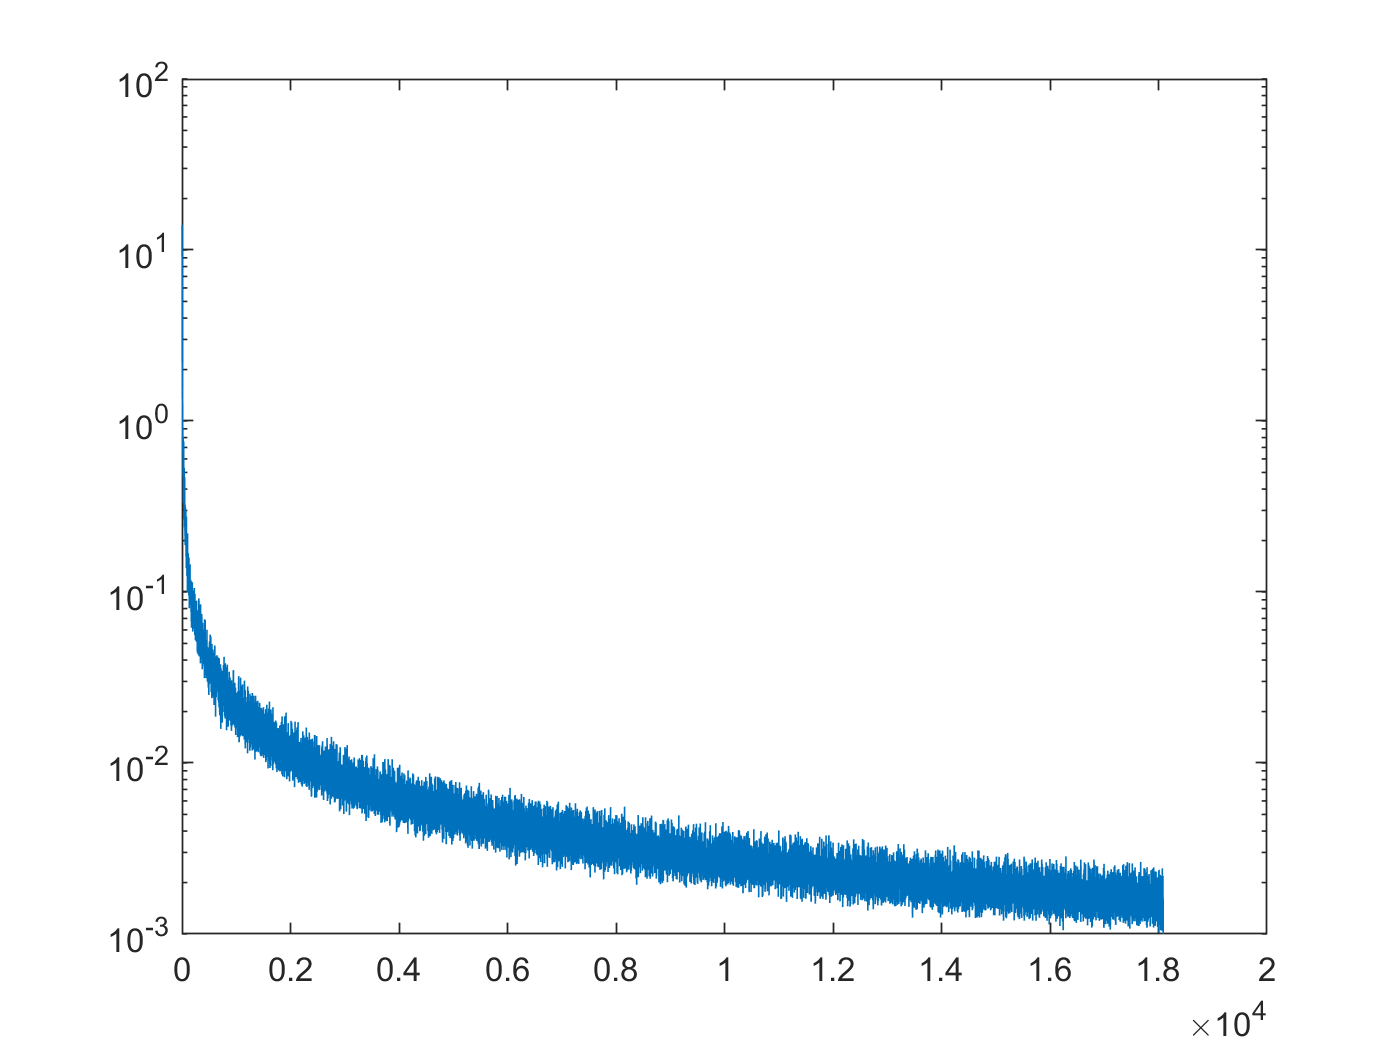
\includegraphics[width=0.8\textwidth]{gaps.png}
    \caption{Plot of the Frank-Wolfe gap versus the number of iterations.}
    \label{fig:my_label}
\end{figure}

\subsection*{Question 14} 
\begin{figure}[h]
    \centering
    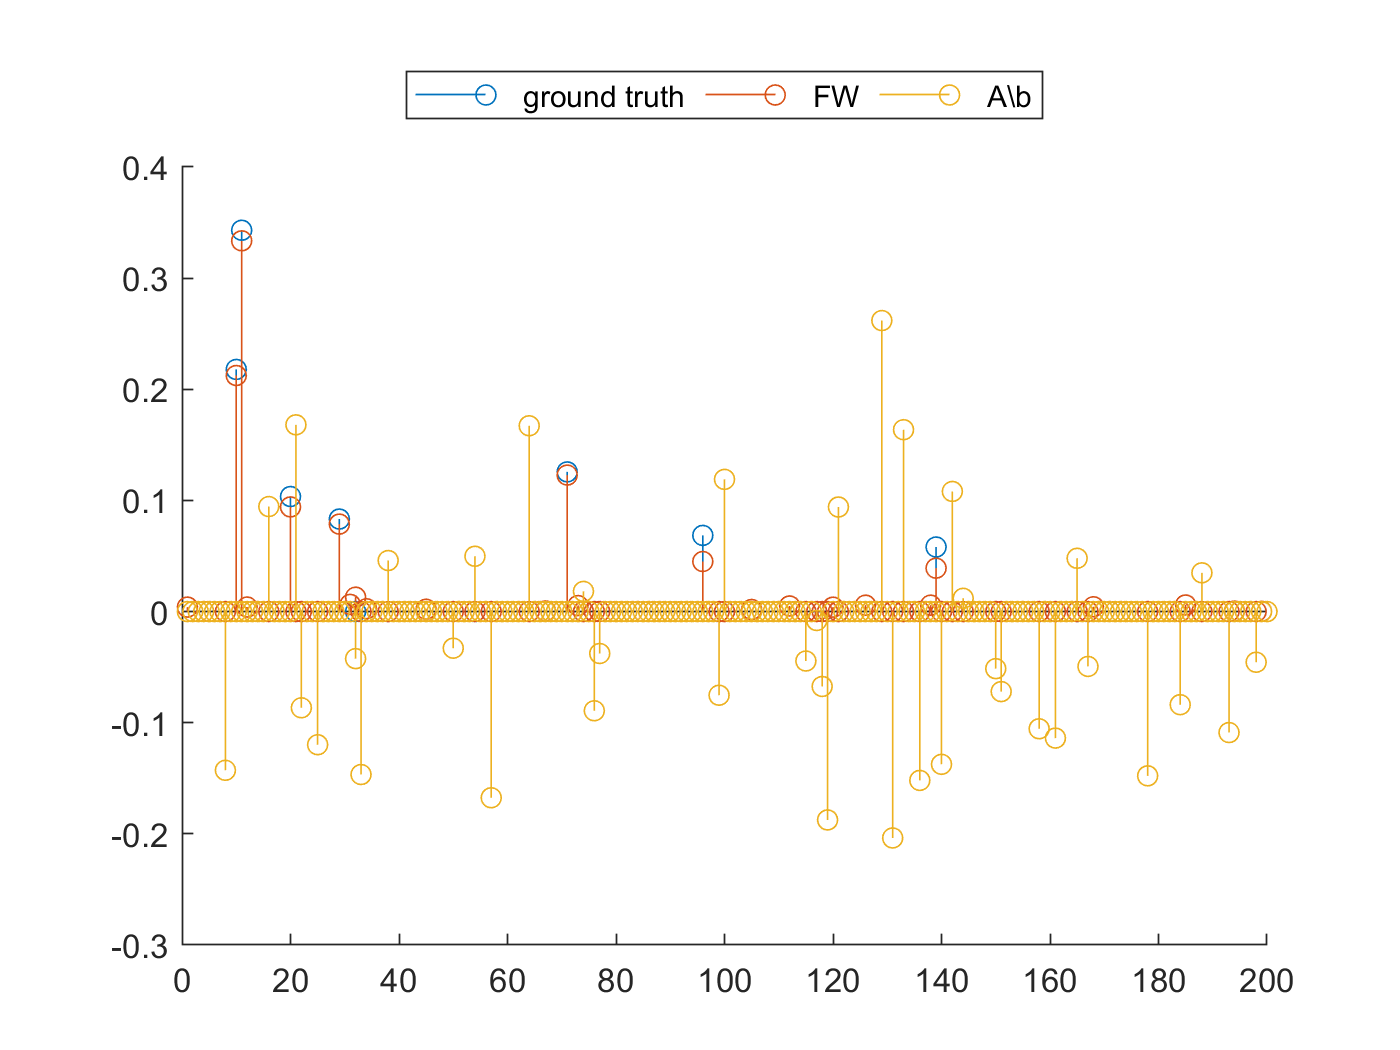
\includegraphics[width=0.5\textwidth]{compare.png}
    \caption{Comparison of the Frank-Wolfe algorithm, the true value and the vector obtained by the Matlab solver.}
    \label{fig:next}
\end{figure}

\newpage

\section*{Part 3 : KKT conditions and constraint qualifications}

\subsection*{Question 1}\hfil\par
Notice that:
\[f_i(x)\leq y;\ \forall \ i=1,\dots,N\iff\]
\[\max_{i=1,\dots,N}f_i(x)\leq y\iff \]
\[f(x)\leq y \implies \]
\[\min_xf(x)\leq\min_{(x,y)\in S}y\]

The other inequality is trivial as \((x,f(x))\in S\). So we can easily conclude that the 2 programs have the same optimal value.

\subsection*{Question 2}\hfil\par
Notice that the constraints for \(S\) are:

\[
    g_i(x,y)=f_i(x)-y\leq 0;\ \forall \ i=1,\dots,N
\]

It is easy to see that:
\[
    \nabla g_i(x,y)=\begin{pmatrix}
    \nabla f_i(x)\\
     -1
    \end{pmatrix}    
\]

The KKT conditions for \((x,y)\in S\) are: \((x,y)\) is a KKT point if there exists \(\lambda\in\mathbb{R}^N\), with \(\lambda\geq0\) such that:
\[
    -(0,\dots,0,1)=   \sum_{i=1}^{N}\lambda_i(\nabla f_i(x)^T,-1)    
\]
and
\[
    \lambda_i(f_i(x)-y)=0;\ \forall\ i=1,\dots,N  
\]
\subsection*{Question 3}\hfil\par
Let \(n=1\) and:
\[
    f_1(x)=x,\ f_2(x)=x^2,\ f_3(x)=x^3
\]

Then:
\[
  \nabla g_1(x,y)=\begin{pmatrix}
    1\\
     -1
    \end{pmatrix},\ \nabla g_2(x,y)=\begin{pmatrix}
    2x\\
     -1
    \end{pmatrix},\ \nabla g_3(x,y)=\begin{pmatrix}
    3x^2\\
     -1
    \end{pmatrix}
\]

For \((x,y)=(1,1)\in S\), it is clear that LICQ doesn't hold as \(\nabla g_1(1,1),\ \nabla g_2(1,1),\ \nabla g_3(1,1)\) are linearly dependent as a family of 3 vectors in \(\mathbb{R}^2\) (\(g_i(1,1)=0\) for all \(i\)).

\subsection*{Question 4}\hfil\par
Let \(I(x,y)=\{i\in\{1,\dots ,N\}\ |\ g_i(x,y)=0\}\). Then for MFCQ to hold, for all \((x,y)\in S\) we need to find a point \((\tilde x, \tilde y)\in S\) such that:
\[
  \langle \nabla g_i(x,  y), (\tilde x- x, \tilde y-y)\rangle<0;\ \forall\ i\in I(x)
\]
Substituting \(\nabla g_i\), we need to find \((\tilde x, \tilde y)\in S\) such that:
\[
    \left\langle \begin{pmatrix}
        \nabla f_i(x)\\
         -1
        \end{pmatrix}    , (\tilde x- x, \tilde y-y)\right\rangle<0;\ \forall\ i\in I(x)
\]
But notice that if we set \(\tilde x:=x\) and \(\tilde y:=y+1\) then:
\[
    \left\langle \begin{pmatrix}
        \nabla f_i(x)\\
         -1
        \end{pmatrix}    , (0, 1)\right\rangle=\langle-1,1\rangle=-1<0;\ \forall\ i\in I(x)
\]

So MFCQ holds for all \((x,y)\in S\).

(\textbf{Note}:\((x,y+1)\in S\) as \(y+1>y\geq f_i(x)\), for all \(i\))
\end{document}
























































